\begin{frame}
\frametitle{Xanadu}
\begin{itemize}
	\item 1960
	\item Langzeitprojekt (Open source in 1999)
	\item Ted Nelson
	\item mehr Framework als Programm
	\item bestehend aus Prototypen und Modelle
	\item "docuverse" - ein elektronische universale Bibliothek
\end{itemize}

\begin{figure}[htbp]
	\centering
	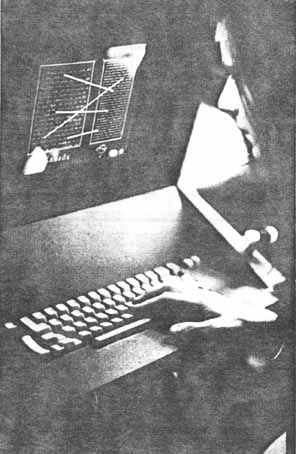
\includegraphics[width=0.22\textwidth]{images/xanadu}
\end{figure}

\end{frame}

\begin{frame}
\frametitle{Xanadu}
\framesubtitle{Funktionen}
\begin{itemize}
	\item Userinterface / Bedienmöglichkeiten
	\begin{itemize}
		\item xxxxx
	\end{itemize}
	\item Links / Strukturen
	\begin{itemize}
		\item Kommentare, Notizen und Verknüpfungen innerhalb der Dokumente zu anderen Dokumenten
	\end{itemize}
\end{itemize}
\end{frame}
